\documentclass{article}




\usepackage{amsmath,amssymb,graphicx,geometry}

\usepackage{xepersian}

\setlength{\parindent}{0mm}
\settextfont{XB Niloofar}


\begin{document}

{
\huge


\begin{center}
به نام او

\begin{table}[h]
\centering
\Large
\begin{tabular}{p{90mm}p{50mm}}
میانترم درس سیگنالها و سیستم ها
&
مدت زمان: 2 ساعت
\\
نام و نام خانوادگی: 
&
شماره دانشجویی:
\end{tabular}
\end{table}
\end{center}
}
\hrulefill

\large

سوال 1) برای هر یک از سیستم های زیر، خواص خطی بودن، علی بودن، معکوس پذیری، پایداری و مستقل از زمان بودن را بررسی کنید.

الف)
$
y(t)=\begin{cases}
x(t)+x(2)\delta(t-1)&,\quad x(t)\ge 0\\
x^2(t-1)&,\quad x(t)< 0
\end{cases}
$

ب) 
$
y[n]=x[n-2]+x[2-n]
$


\newpage

سوال 2) اطلاعات زیر در مورد یک سیگنال متناوب
$
x(t)
$
با دوره تناوب
$
2\pi
$
و ضرایب سری فوریه‌ی 
$
a_k
$
داده شده است:
\begin{itemize}
\item
سیگنال 
$
x(t)
$
حقیقی و دارای 5 ضریب سری فوریه است.
\item
پاسخ سیستمی خطی و مستقل از زمان با پاسخ ضربه‌ی 
$
\frac{\sin \frac{3}{2}t}{\pi t}
$
به ورودی 
$
x(t)
$،
برابر
$
1+2\cos t
$
است.
\item
$
\sum_{k=-2}^{2}|a_k|^2=\frac{7}{2}
$
\end{itemize}
در این صورت، سیگنال 
$
x(t)
$
را بیابید.

\newpage

سوال 3) سیگنال 
$
x(t)
$
به صورت زیر است:
\begin{figure}[h]
\centering
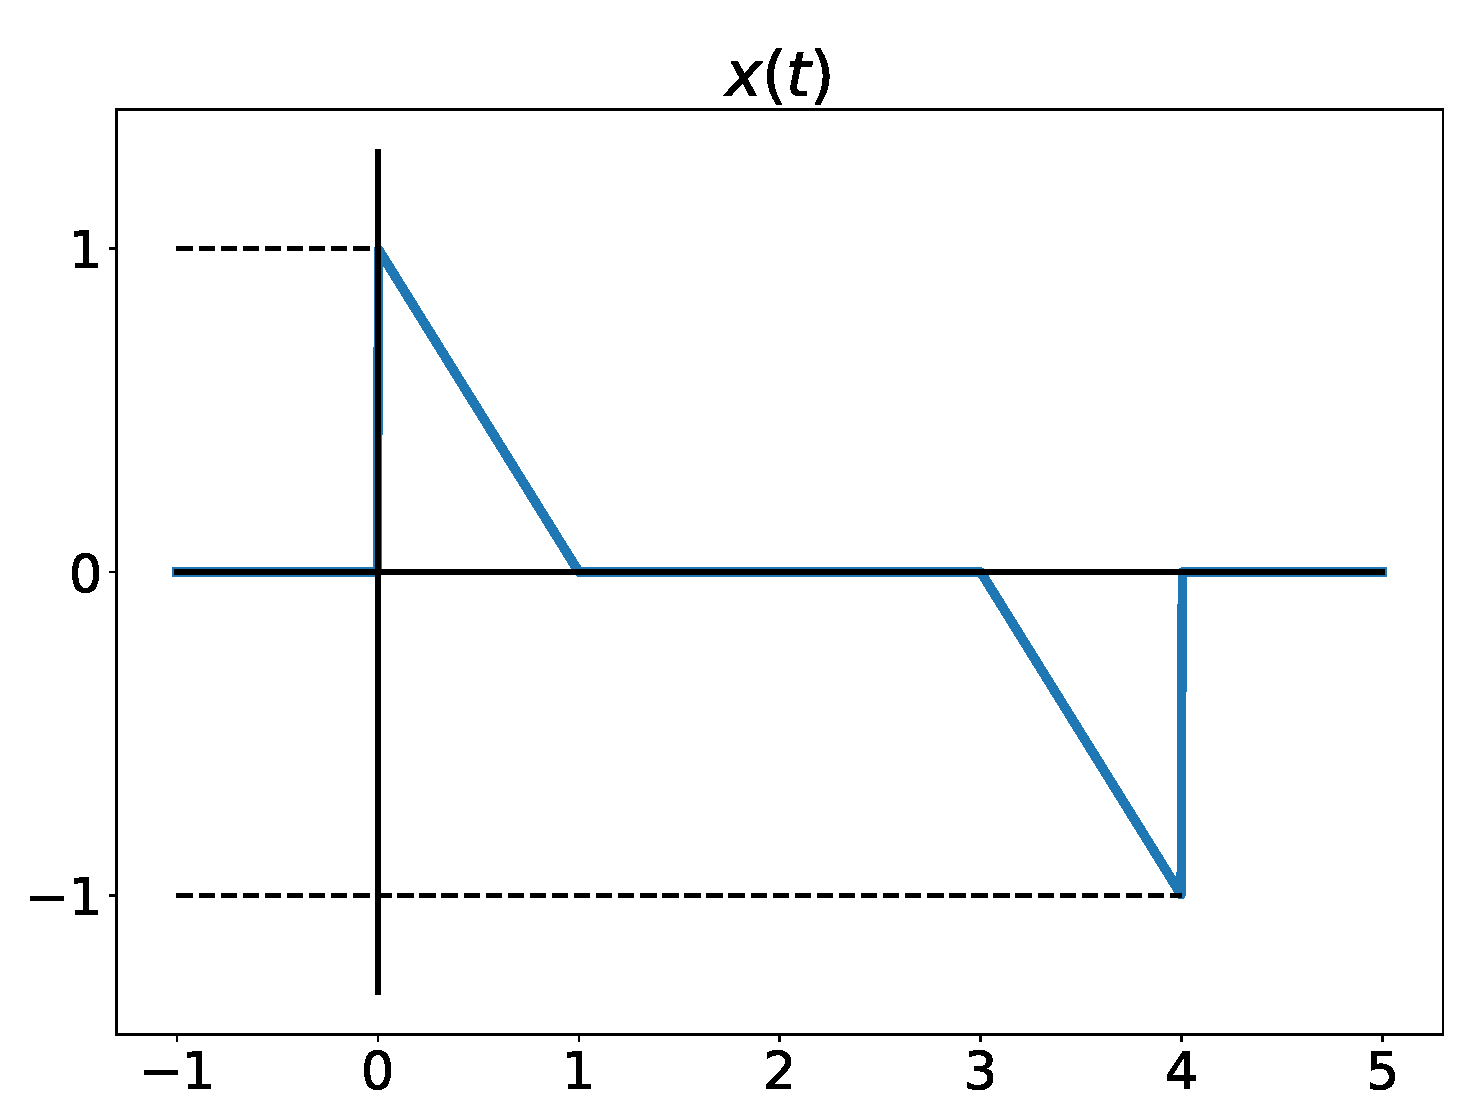
\includegraphics[width=80mm]{midterm_q3.eps}
\end{figure}

اگر تبدیل فوریه‌ی این سیگنال برابر 
$
X(j\omega)
$
باشد،

الف) 
$
\measuredangle X(j\omega)
$
را بیابید.

ب)
$
X(j0)
$
را بیابید.

پ)
$
\int_{-\infty}^{\infty}X(j\omega)\frac{2\sin\omega}{\omega}e^{j\omega}d\omega
$
را بیابید.

ت) عکس تبدیل فوریه‎ی
$
\mathrm{Re}\{X(j\omega)\}
$
را رسم کنید.

\newpage

سوال 4) اطلاعات زیر در خصوص یک سیستم خطی، مستقل از زمان و حقیقی با تابع انتقال 
$
H(s)
$
داده شده است:

\begin{itemize}
\item
تابع انتقال سیستم دارای 3 قطب محدود و 1 صفر محدود است.
\item
یکی از قطب ها در 
$
s=-1+j
$
است.
\item
پاسخ سیستم به ورودی 
$
e^tu(-t)
$
برابر صفر و به ورودی
$
e^{2t}
$
برابر
$
\frac{1}{15}e^{2t}
$
است.
\item
برای این سیستم داریم
$
\int_{-\infty}^{\infty}h(t)dt=-1
$
.
\end{itemize}

الف) پاسخ ضربه‌ی این سیستم و سیستم معکوس را بیابید.

ب) پایداری و علی بودن سیستم معکوس را بررسی کنید.

\newpage

سوال 5)  فرض کنید حداقل فرکانس نمونه برداری از سیگنال 
$
x(t)
$
با تبدیل فوریه‌ی 
$
X(j\omega)
$
طبق قضیه‌ی نمونه برداری برابر
$
\omega_0
$
باشد. در این صورت، حداقل فرکانس نمونه برداری هر یک از سیگنال های زیر را (به گونه ای که طبق قضیه‌ی نمونه برداری، همپوشانی رخ ندهد) به دست آورید.

الف) 
$
x^2(t)\cos\omega_0 t
$

ب)
$
x(\frac{t}{2})
$

پ)
$
x(t)+x(t-1)
$

ت)
$
x(t)*\frac{\sin \frac{\omega_0}{6}t}{\omega_0t}
$
(منظور از $*$ عملگر کانولوشن است.)

\end{document}